% Supplementary update (19 October 2026) to the ARC Prize Research Summit poster: CORA reasoning v2.
% Every number is indexed in records/CORA_SUMMIT_CLAIM_LEDGER_20261017.md (rows 18-21).
% Figure: scripts/summit_figures.py -> docs/summit_poster/figures/fig_v2_uncertified_00dbd492.png (pinned inputs).
\documentclass[10pt]{article}
\usepackage[a4paper, margin=1.5cm]{geometry}
\usepackage[scaled]{helvet}
\renewcommand{\familydefault}{\sfdefault}
\usepackage[T1]{fontenc}
\usepackage{microtype}
\usepackage{graphicx}
\usepackage{xcolor}
\usepackage{enumitem}
\setlist{nosep, leftmargin=1.3em}
\definecolor{ink2}{HTML}{52514E}
\definecolor{critical}{HTML}{D03B3B}
\pagestyle{empty}
\pdftrailerid{}
\setlength{\parskip}{0.35em}
\setlength{\parindent}{0pt}
\raggedright

\begin{document}
{\large\bfseries Supplement, 19 October: when a fitting hypothesis is not enough\par}
{\color{ink2} CORA reasoning v2, a development update for the summit poster. It is not part of any Kaggle entry, and
nothing here is certified.\par}

\textbf{What v2 does.}
\begin{itemize}
  \item A hypothesis is a triple: an object representation (one of CORA's seven segmentations), a geometry (one of
        37,750 growth expressions) and a colour policy.
  \item v2 keeps \emph{every} hypothesis that reproduces every demonstration exactly, predicts the test with each, and
        abstains when they disagree.
  \item It reruns the whole search with each demonstration held out, and certifies only a unique prediction that every
        fold rebuilds. The verifier is CORA's unchanged leave-one-out discipline.
\end{itemize}

\textbf{Typed diagnoses.} When the hypotheses are not enough, v2 records:
\begin{itemize}
  \item the symptom (8 labels);
  \item the competing causes;
  \item a bounded probe on the demonstrations, and its result;
  \item what stays uncertain, and the next action.
\end{itemize}
It reads no test answer. \emph{No program found} is never reported as \emph{new semantics needed}.

\begin{center}
  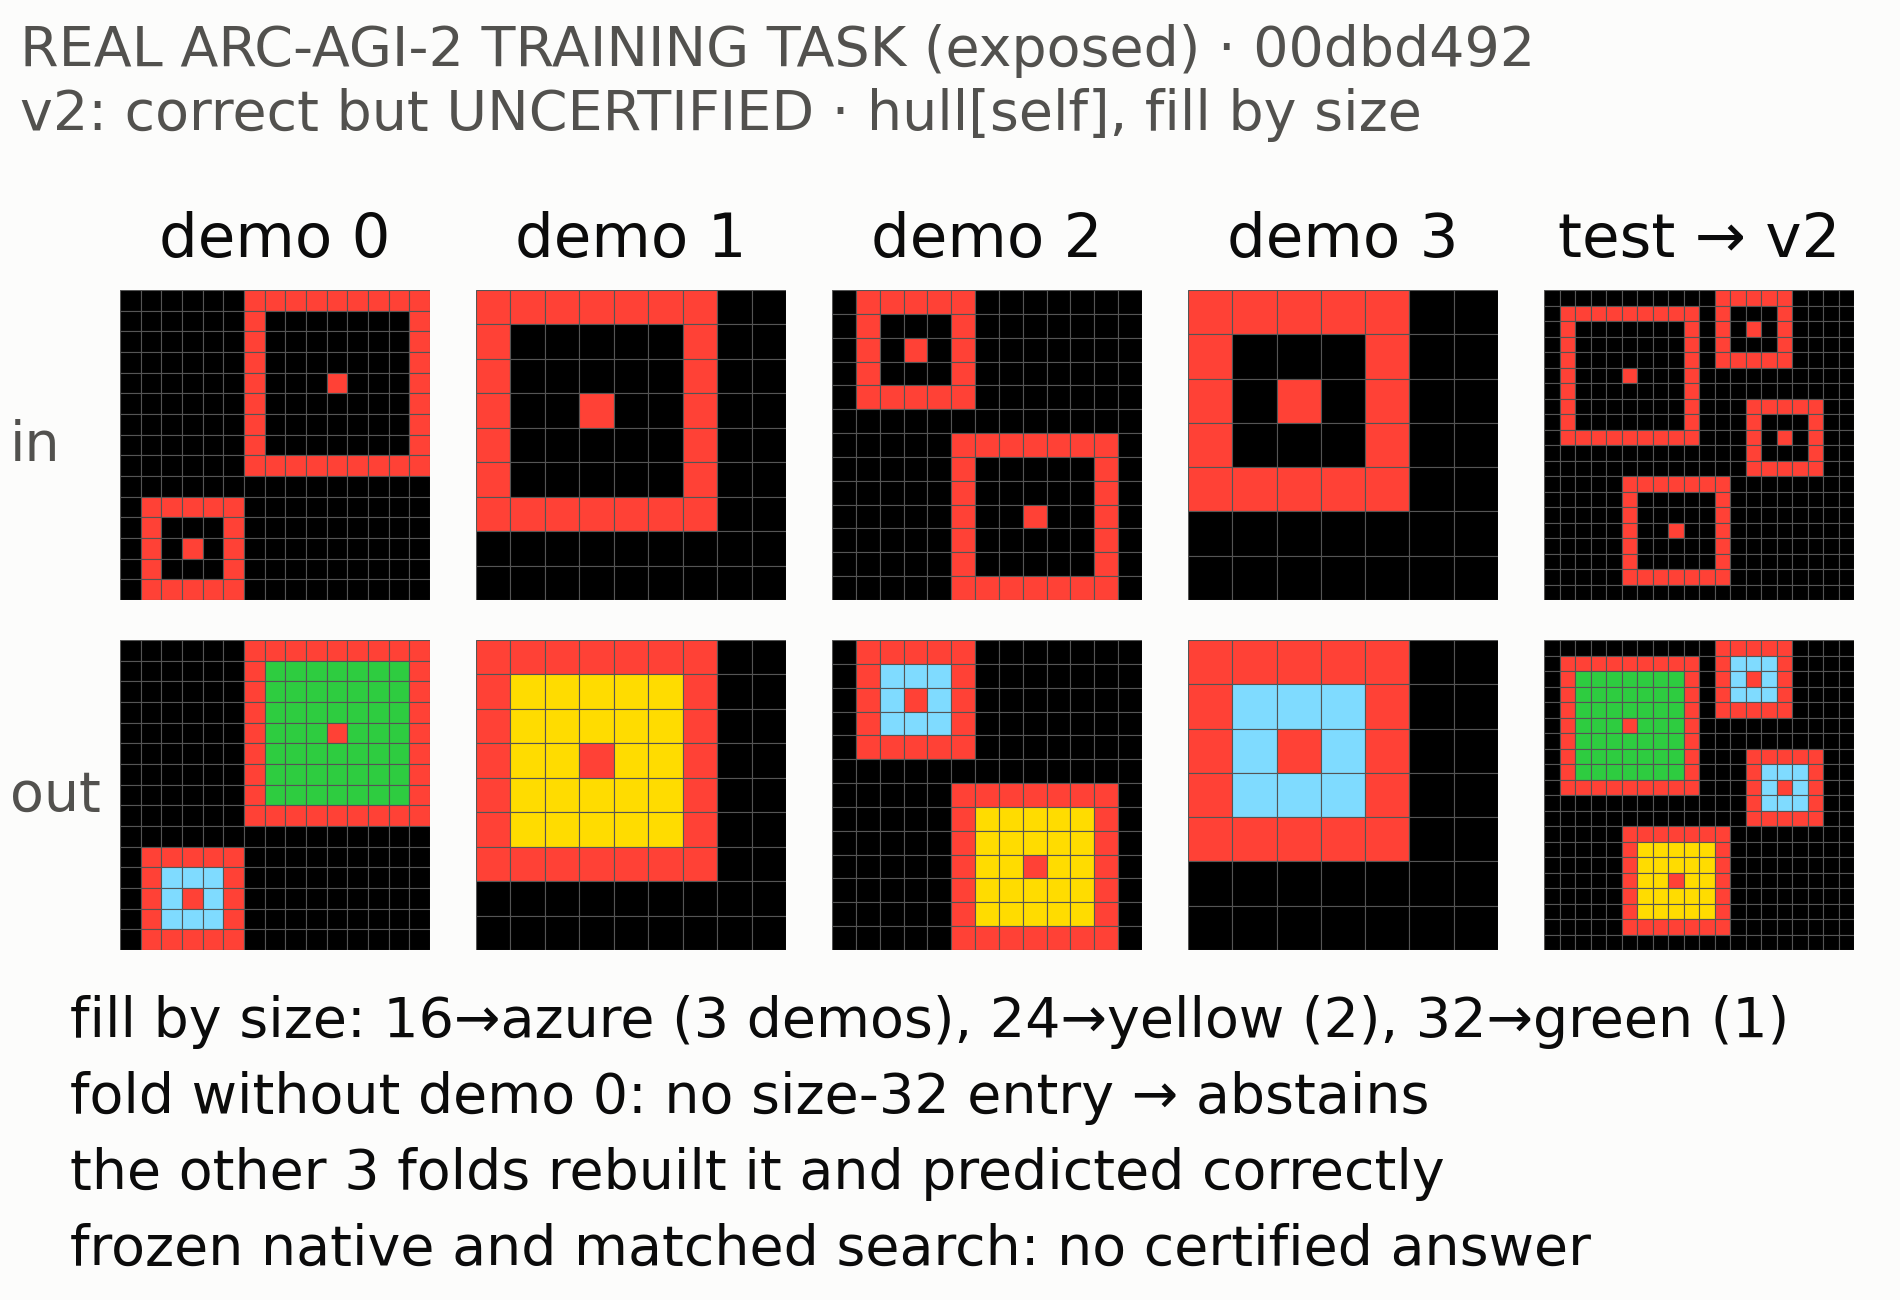
\includegraphics[width=0.64\linewidth]{../summit_poster/figures/fig_v2_uncertified_00dbd492.png}
\end{center}

\textbf{The first correct but uncertified prediction (00dbd492, an exposed training task).} v2 fills each frame with a
colour set by its size. Its 1,365 consistent hypotheses all agree, and the prediction is correct. Frozen CORA and matched
extra search give no certified answer.
\begin{itemize}
  \item \textbf{Why certification fails:} the test needs the size-32 colour, which only one demonstration shows, so
        the fold without that demonstration abstains.
  \item \textbf{What the diagnosis rules out:} the probes reject ambiguity, a representation error and a defect. The
        cause is insufficient evidence.
  \item \textbf{What it does not change:} a failure-blind reasoner with the same language gives the same answer. This
        is candidate generation; it does not show that diagnosis helps.
\end{itemize}

\textbf{Engineering runs (exposed tasks, in-sample).} \begin{itemize}
  \item \textbf{58 pool tasks:} 0 certified; 3 correct and 1 wrong exploratory predictions. Added to native's recorded
        Kaggle-path attempts, they would raise the two-attempt count from 7 to 8 (filling only duplicate attempt-2 slots)
        or to 9 (always as attempt 2), with none lost.
  \item \textbf{60 development tasks:} 0 certified; 1 correct exploratory prediction, on a task native already solves
        (12 stays 12).
  \item \textbf{Main limitation:} 32 of the 60 change cells in ways v2 cannot express (several actions, or recolouring
        or deletion only). That is the next hypothesis class to build.
\end{itemize}

\textbf{{\color{critical}Not shown.}}
\begin{itemize}
  \item No certified v2 answer.
  \item No result on tasks outside development.
  \item No evidence that diagnosis-driven revision beats failure-blind revision.
\end{itemize}

\textbf{Next.} A frozen real-task test: v2, frozen CORA and matched search, then revision chosen by the authentic
diagnosis, failure-blind and shuffled. It waits for a cohort check, because Step B's protected splits are drawn from
the same training file.

{\color{ink2}\small Sources: \texttt{records/CORA\_REASONING\_V2\_*\_20261019.md}; ledger rows 18--21.\par}
\end{document}
